Целью работы в курсовой работе стало написание программного модуля, осуществляющего отображения состояния работы сервиса.

\subsubsection{Принцип работы}

Программа реализована с использованием микрофреймворка flask. Программный модуль получает данные из базы данных, выводит результат состояний работы сервисов каждой команды на html страницу.

При инициализации модуля есть возможность устанавливать порт, на котором будет работать модуль.

Доступ к модулю осуществляется через браузер, например по ссылке http://127.0.0.1:9000  
Пример работы модуля приведен на рисунке ниже.
\begin{figure}[h!]
\center{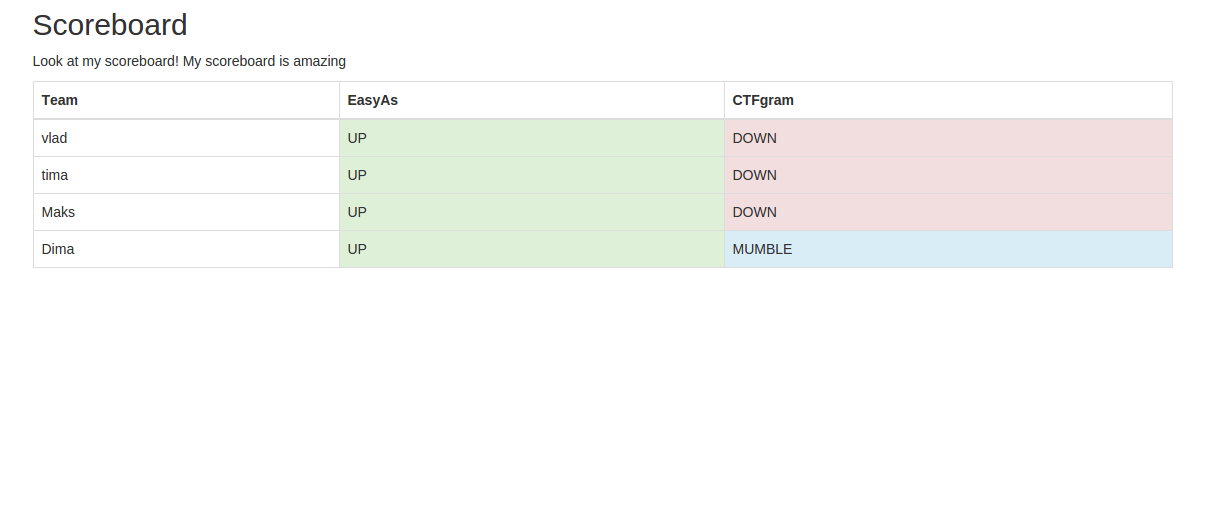
\includegraphics[width=1\linewidth]{images/score_sample.png}}
\caption{Пример работы scoreboard.py}
\end{figure}

Ниже представлена схема работы scoreboard.py

\begin{figure}[h!]
\center{\includegraphics[width=0.25\linewidth]{individual_reports/score.png}}
\caption{Cхема работы scoreboard.py}
\end{figure}

\clearpage